\newpage
\section{Analyse}
\subsection{Product backlog}
\noindent\adjustbox{max width=\textwidth}{
\begin{tabular}{| p{1cm} | p{16cm} |}
	\hline
	US-01 & En tant qu'utilisateur je voudrais savoir mon score.\\
	\hline
	US-02 & En tant qu'utilisateur je voudrais savoir si j'ai bien répondu.\\
	\hline
	US-03 & En tant qu'utilisateur je voudrais savoir si j'ai mal répondu.\\
	\hline
	US-04 & En tant qu'utilisateur je voudrais savoir quelle était la bonne réponse.\\
	\hline
	US-05 & En tant qu'utilisateur je voudrais savoir mettre mon jeu sur pause.\\
	\hline
	US-06 & En tant qu'utilisateur je voudrais savoir reprendre mon jeu où je l'avait laissé.\\
	\hline
	US-07 & En tant qu'utilisateur je voudrais savoir arrêter mon jeu à tout moment.\\
	\hline
	US-08 & En tant qu'utilisateur j'aimerais joué en multi joueur localement.\\
	\hline
	US-09 & En tant qu'administrateur je dois pouvoir ajouter une nouvelle carte au deck.\\
	\hline
	US-10 & En tant qu'administrateur je veux pouvoir supprimer une carte du deck.\\
	\hline
	US-11 & En tant qu'administrateur je veux pouvoir modifier une carte existante.\\
	\hline
	US-12 & En tant qu'utilisateur j'aimerais avoir une musique de fond.\\
	\hline
	US-13 & En tant qu'utilisateur j'aimerais pouvoir gérer le volume de la musique.\\
	\hline
	US-14 & En tant qu'utilisateur j'aimerais pouvoirs activer ou désactiver la musique de fond.\\
	\hline
	US-15 & En tant qu'utilisateur je voudrais pouvoir choisir mon propre pseudonyme.\\
	\hline
	US-16 & En tant qu'utilisateur je voudrais voir un plateau de jeu.\\
	\hline
	US-17 & En tant qu'utilisateur je voudrais avoir mon pion.\\
	\hline
	US-18 & En tant qu'utilisateur je voudrais savoir reconnaitre mon pion.\\
	\hline
	US-19 & En tant que joueur, je voudrais communiquer avec d'autre joueurs.\\
	\hline
	US-20 & En tant que joueur, j'aimerais jouer avec d'autre joueurs en ligne.\\
	\hline
	US-21 & En tant que joueur, j'aimerais rejoindre une partie en ligne.\\
	\hline
	US-22 & En tant que joueur, j'aimerais héberger une partie en ligne.\\
	\hline
\end{tabular}
}

\newpage
\subsection{Les classes}

\subsubsection{Le modèle}
\begin{figure}[h]
	\centering
	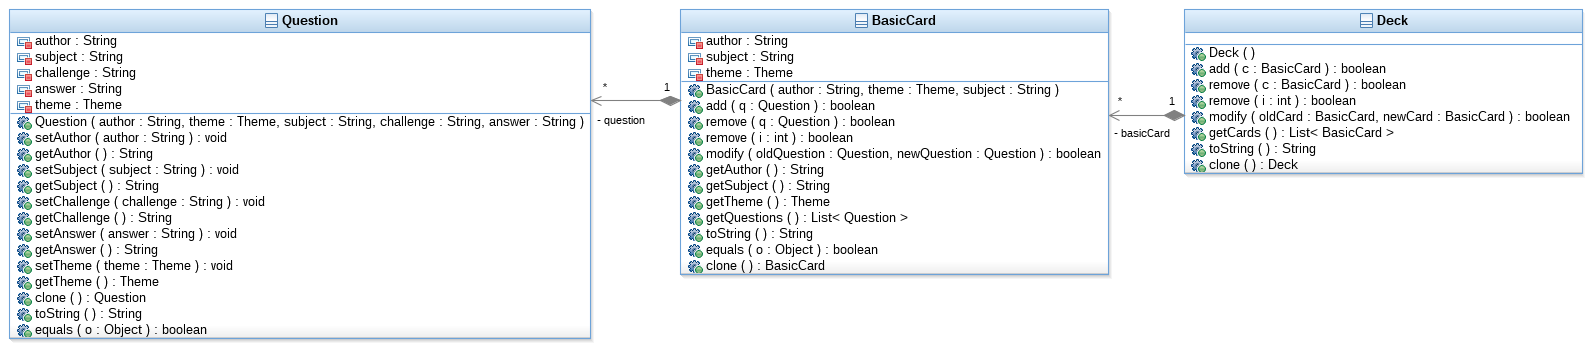
\includegraphics[width=\textwidth]{ttmc_modele.png}
	\caption{Diagramme du modèle}
	\label{fig:diag_modele}
\end{figure}

\subsubsection{La vue}
\begin{figure}[h]
	\centering
	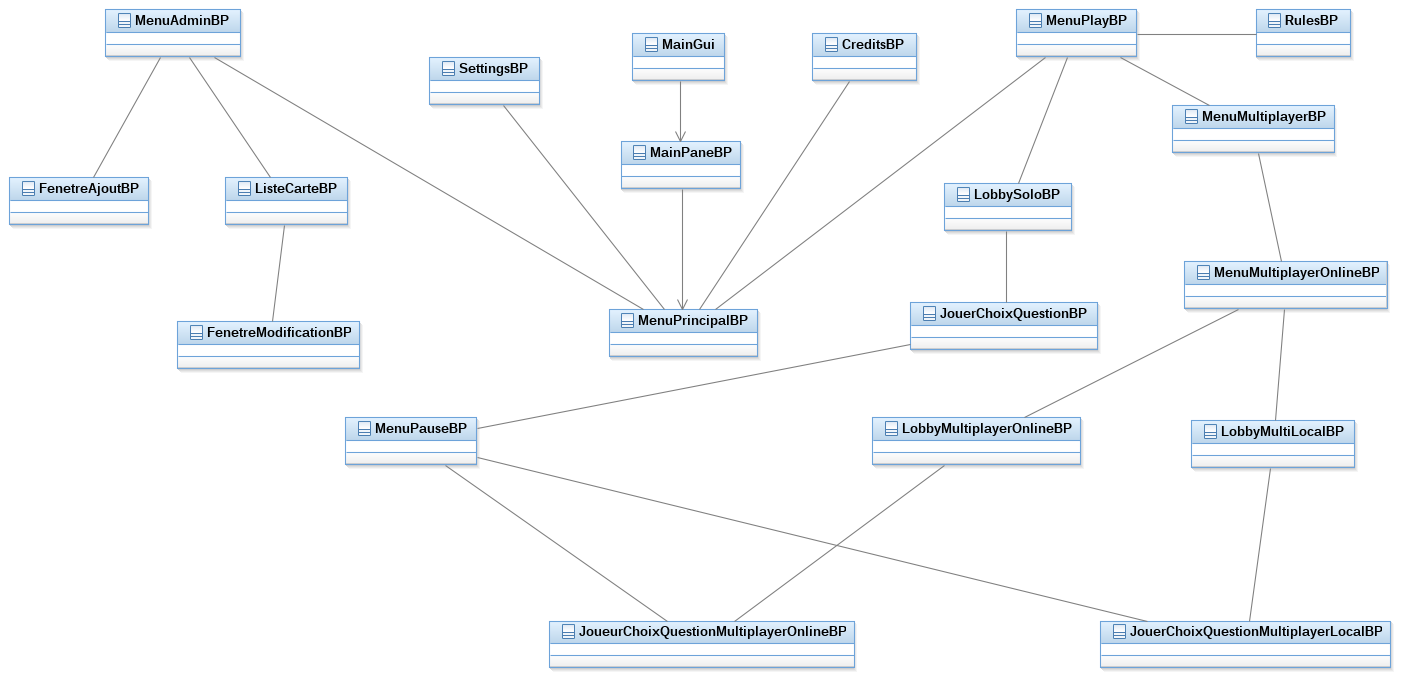
\includegraphics[width=\textwidth]{ttmc_vue.png}
	\caption{Diagramme de la vue}
	\label{fig:diag_vue}
\end{figure}

\subsubsection{Les exceptions}
